% This is a Beamer LaTeX template for the STFC Hartree Centre using the May 2021 brand identity.
% Written by Viktor Zolyomi.
\documentclass[english]{beamer}
\usepackage{helvet}
\renewcommand{\familydefault}{\sfdefault}
\usepackage[T1]{fontenc}
\usepackage[latin9]{inputenc}
\usepackage{amssymb}
\usepackage{physics}
\usepackage{hyperref}

\makeatletter
%%%%%%%%%%%%%%%%%%%%%%%%%%%%%% Textclass specific LaTeX commands.
% this default might be overridden by plain title style
\newcommand\makebeamertitle{\frame{\maketitle}}%
% (ERT) argument for the TOC
\AtBeginDocument{%
  \let\origtableofcontents=\tableofcontents
  \def\tableofcontents{\@ifnextchar[{\origtableofcontents}{\gobbletableofcontents}}
  \def\gobbletableofcontents#1{\origtableofcontents}
}

%%%%%%%%%%%%%%%%%%%%%%%%%%%%%% User specified LaTeX commands.
%\usetheme{Warsaw}
\usetheme{Darmstadt}
% or ...

    \usefonttheme{structurebold}
    \setbeamerfont{title}{series=\bfseries,parent=structure}
    \setbeamerfont{subtitle}{size=\scriptsize,series=\bfseries,parent=structure}
    \setbeamerfont{author}{size=\scriptsize,series=\bfseries,parent=structure}
    \setbeamerfont{institute}{size=\scriptsize,series=\bfseries,parent=structure}
    \setbeamerfont{date}{size=\scriptsize,series=\bfseries,parent=structure}

\setbeamercovered{transparent}
% or whatever (possibly just delete it)

\usepackage{caption}
\usepackage[absolute,overlay]{textpos}
\setbeamertemplate{footline}[frame number]
\usepackage{graphbox}

\beamertemplatenavigationsymbolsempty
\setbeamertemplate{headline}{}

\setbeamertemplate{footline}{

\includegraphics[align=c,height=0.9cm]{UKRI_STFC_HARTREE_CENTRE_RGB.png}
\hfill
\usebeamercolor[fg]{page number in head/foot}
\usebeamerfont{page number in head/foot}
\insertframenumber\,/\,\inserttotalframenumber\kern1em
}
\definecolor{bluegreen}{RGB}{3, 166, 155}
%\definecolor{newblue}{RGB}{18, 18, 38}
%\definecolor{newgray}{RGB}{40, 40, 40}
\definecolor{newbluegreen}{RGB}{0, 190, 213}
\definecolor{newblue}{RGB}{0, 48, 136}
\definecolor{newgray}{RGB}{103, 103, 103}
\definecolor{newred}{RGB}{255, 90, 90}
\definecolor{newlightblue}{RGB}{30, 93, 248}
\definecolor{newdarkblue}{RGB}{46, 45, 98}
%\setbeamercolor{frametitle}{bg=bluegreen, fg=white}
%\setbeamercolor{title}{bg=bluegreen, fg=white}
\setbeamercolor{normal text}{fg=newgray}

% %%%%%%%%%%%%%%%%%%%%%%%%
%    TITLE PAGE OPTIONS
% %%%%%%%%%%%%%%%%%%%%%%%%
%
% comment out the following lines if you prefer a rounded box in the title along with drop shadows:
\setbeamertemplate{frametitle}[default]
\setbeamertemplate{title page}[default][colsep=-4bp,rounded=false]
% comment out the above line (i.e. only the title page line) and uncomment the one below for rounded box without shadow:
%\setbeamertemplate{title page}[default][colsep=-4bp,rounded=true]
%
% uncomment the 2 lines below and comment out the 2 lines below them for white title on blue background:
%\setbeamercolor{title}{bg=newblue,fg=white}
%\setbeamercolor{frametitle}{bg=newblue, fg=white}
% comment out the above 2 lines and uncomment the 2 below for blue title on white:
\setbeamercolor{title}{bg=white,fg=newblue}
\setbeamercolor{frametitle}{bg=white,fg=newblue}
%
% %%%%%%%%%%%%%%%%%%%%%%%%

\title{Shor's algorithm}
\author{Dilhan Manawadu}
\date{\today}

\makeatother

\usepackage{babel}
\begin{document}
{   \usebackgroundtemplate{{ 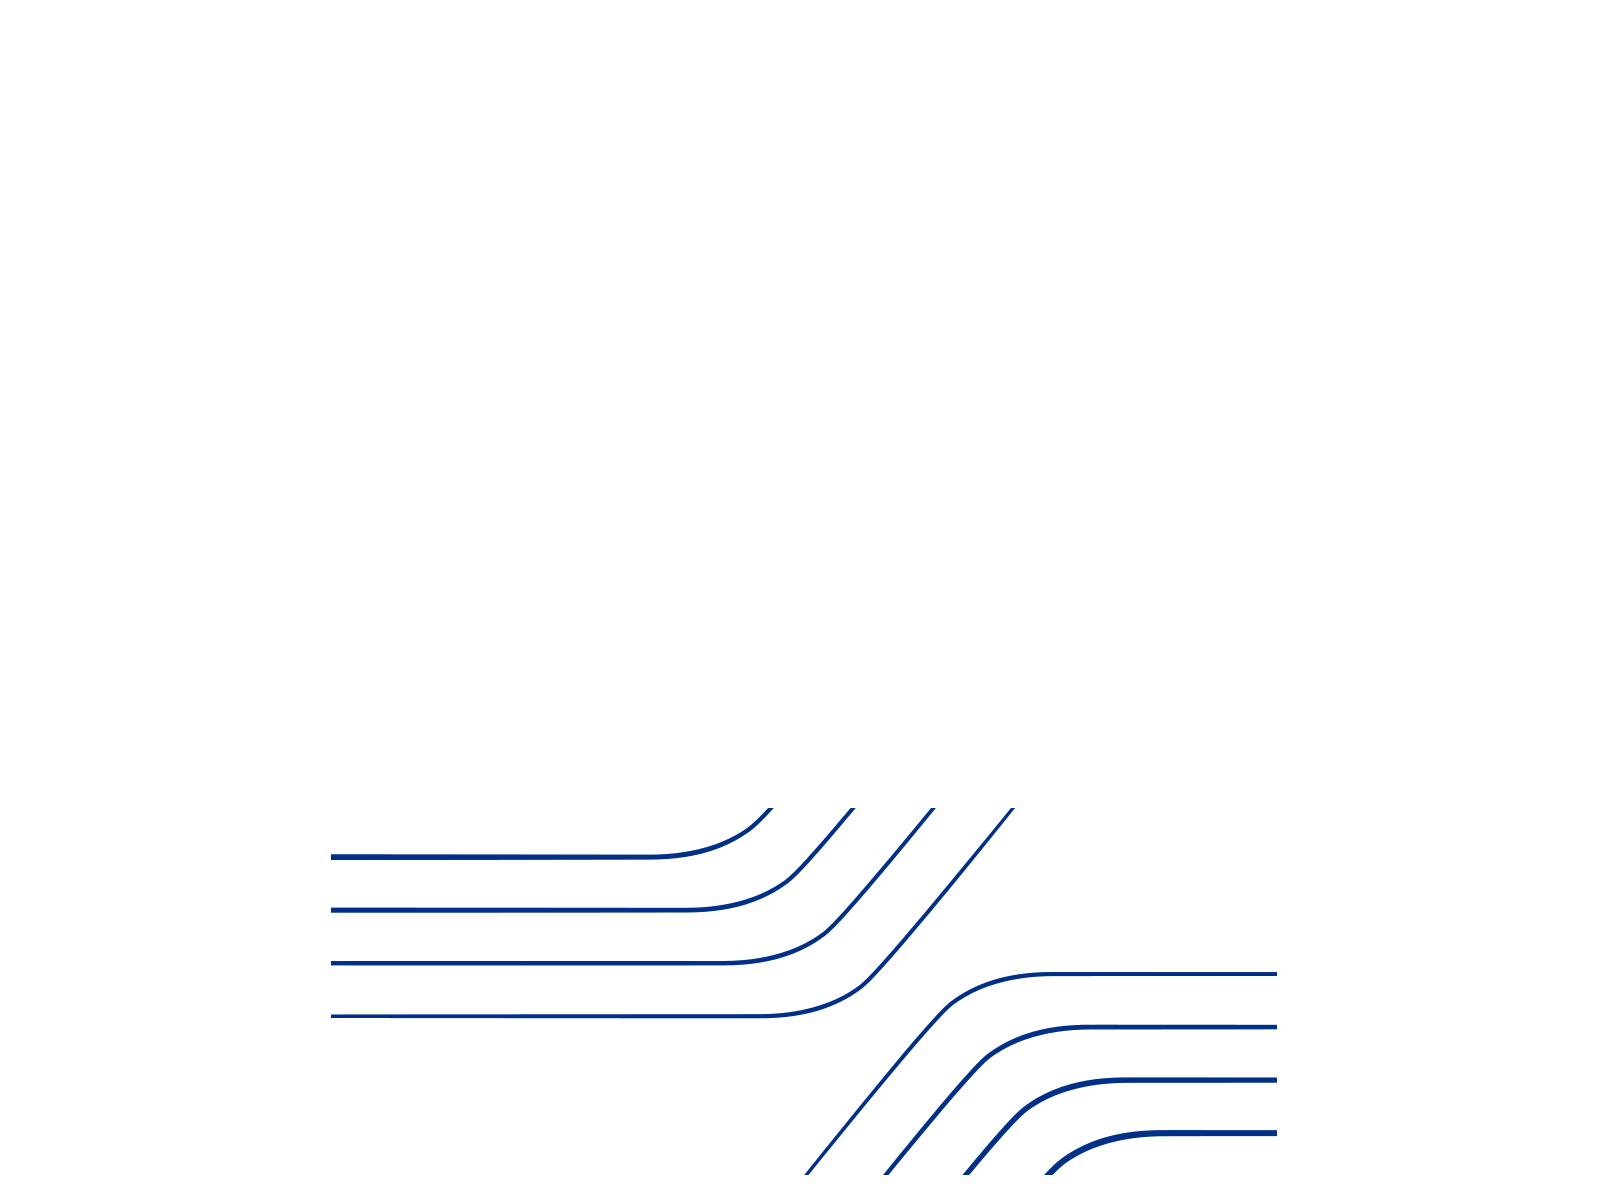
\includegraphics[width=1.05\paperwidth]{Pattern.png}}}   \begin{frame}     \titlepage   \end{frame} }

%\pgfdeclareimage[height=0.5cm]{institution-logo}{UKRI_STFC_HARTREE_CENTRE_RGB.png}
%\logo{\pgfuseimage{institution-logo}}

%\AtBeginSubsection[]{%
%  \frame<beamer>{ 
%    \frametitle{Outline}   
%    \tableofcontents[currentsection,currentsubsection] 
%  }
%}

%\beamerdefaultoverlayspecification{<+->}




\section{Factoring large numbers}

\begin{frame}{\textbf{Factoring large numbers}}

\begin{itemize}
\item A prime number is a natural number greater than 1 that is divisible by only 1 and itself.
\item By multiplying two prime numbers, we can generate composite numbers with two prime factors. For example $21 = 3 \times 7$.
\item Given a large composite number, can one devise an algorithm to find its prime factors?
\item Shor's algorithm is a quantum algorithm proposed to solve this problem.

\end{itemize}
\end{frame}

\section{Period Finding}

\begin{frame}{\textbf{Factoring large numbers}}

\begin{itemize}
\item The periodic function $f(x)$ is defined by
\begin{equation}
	f(x) = a^x \mod N
\end{equation}
where $\mod N$ stands for division modulo $N$. For example,
\begin{equation}
	11 = 3 \mod 4 \notag
\end{equation}
since $11 \divisionsymbol 4$ returns 3 as the remainder.
\item The period of function $f(x)$ is defined as the smallest non-zero integer $r$ such that $f(r) = a^r \mod N = 1$.
\item A unique $r>0$ exists as long as $a<N$, and $a$ and $N$ do not have common factors, i.e., $\gcd(a,N)=1$ 


\end{itemize}
\end{frame}



\begin{frame}{\textbf{Shor's unitary operator}}

\begin{itemize}
\item Let's define the operator $U$ by
\begin{equation}
	U \ket{y} = \ket{ay\mod N}
\end{equation}
\item For example, $U$ for the periodic function $f(x) = 7^x \mod 15$ is given by,
\begin{equation}
	U \ket{y} = \ket{7 y\mod 15} \notag 
\end{equation}


\item Starting with $y=1$, we get
	\begin{align}
		U \ket{1} &= \ket {7 \mod 15} = \ket{7} \notag \\
U^2 \ket{1} &= U \ket{7}= \ket {49 \mod 15} = \ket{4} \notag  \\
U^3 \ket{1} &= U \ket{4}= \ket {28 \mod 15} = \ket{13} \notag \\
U^4 \ket{1} &= U \ket{13}= \ket {91 \mod 7} = \ket{1} \notag 
	\end{align}
\item Since $U^4\ket{1}=\ket{1}$, $U$ is a unitary operator. 
\item $\{ \ket{7}, \ket{4}, \ket{13}, \ket{1} \}$ forms a basis for $U$.

\end{itemize}
\end{frame}

\begin{frame}{\textbf{Eigenstates of $U$}}

\begin{itemize}
\item Let's define as $\ket{u_0}$ the state created by symmetric superposition of these basis states.
\begin{align}
\ket{u_0}
    &=
        \frac{1}{2} \left (
                \ket{1} + \ket{7} + \ket{4} + \ket{13}
        \right ) \notag  \\
U\ket{u_0}
    &=
        \frac{1}{2} \left (
                U\ket{1} + U\ket{7} + U\ket{4} + U\ket{13}
        \right ) \notag \\
U\ket{u_0}
    &=
        \frac{1}{2} \left (
                \ket{7} + \ket{4} + \ket{13} + \ket{1}
        \right )  \notag \\
U\ket{u_0}
        &=
                \ket{u_0} \notag
\end{align}
$\ket{u_0}$ is an eigenstate of operator $U$.

\end{itemize}
\end{frame}

\begin{frame}{\textbf{Eigenstates of $U$}}

\begin{itemize}
\item Any state $\ket{u_s}$ defined for $s<r $ by
\begin{equation}
	\ket{u_s}
        =
                \frac{1}{\sqrt{r}} \sum_{k=0}^{r-1} \exp{\left (-\frac{2 \pi i s k}{r} \right )} U^k\ket{1}
\end{equation}
is an eigenstate of the operator $U$,
\begin{equation}
	U \ket{u_s}
                =
                        \exp{\left(\frac{2 \pi i s}{r}\right)} \ket{u_s}
\end{equation}
\item If we can prepare the state $\ket{u_s}$ on a quantum computer, we can approximate the value of $r$ using the quantum phase estimation (QPE) algorithm.  
\item We cannot prepare the state $\ket{u_s}$ without knowing $r$!
\end{itemize}
\end{frame}

\begin{frame}{\textbf{Initial state for QPE}}

\begin{itemize}

\item If we sum over states $\ket{u_s}$ for values $0 \le s < r$, the phases cancel to give
\begin{equation}
        \frac{1}{\sqrt{r}} \sum_{k=0}^{r-1} \ket{u_s}
        	=
	\ket{1}
\end{equation}
\item Therefore we can use the easy-to-prepare state $\ket{1}$ as the initial target state for QPE. 
\item As $\ket{1}$ is a symmetric superposition of states $\ket{u_s}$, QPE will measure a phase $\phi = \frac{s}{r}$ where $s$ will be a random integer between 0 and $r-1$ drawn from a uniform distribution.
\end{itemize}


\end{frame}

\begin{frame}{\textbf{Example : Finding $r$ of $a^r \mod 15$ using QPE}}
	
\begin{figure}
	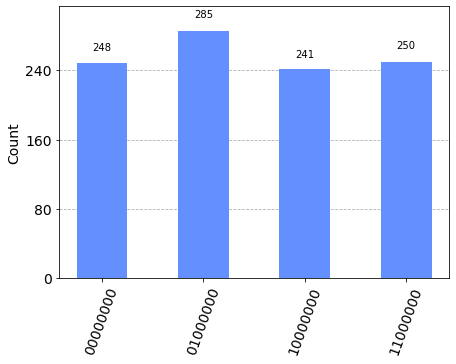
\includegraphics[width=0.4\textwidth]{figs/output}
\end{figure}
\begin{tabular}{|l|c|c|c|c|}
\hline
Register Output (binary) & Decimal & Phase & Fraction \\
\hline
00000000 & $0$ & $\frac{0}{256} = 0.00$ & 0\\
01000000 & $64$ & $\frac{64}{256} = 0.25$ &1/\textbf{4}\\
10000000 & $128$ & $\frac{128}{256} = 0.50$ & 1/2\\
11000000 & $192$ & $\frac{192}{256} = 0.75$ & 3/\textbf{4}\\
\hline
\end{tabular}

\begin{itemize}
\item We find the correct period $r=4$ with $50\%$ accuracy.
\item This is a consequence of using $\ket{1}$ instead of $\ket{u_s}$ to initialise the target registry.
\end{itemize}

\end{frame}

\begin{frame}{\textbf{Factoring}}

\begin{itemize}

\item	Since $r=4$ is even, we can write
\begin{align}
	a^r \mod N &=1 \notag \\
    a^r - 1 &= xN \notag  \\
    (a^{r/2}-1)(a^{r/2}+1) &= xN \notag 
\end{align}
\item we can see that $a^{r/2} \pm 1$ is highly likely to share a factor with $N$.
\item Therefore, we can guess the greatest common dividers of these two integers with N to be a factor of N.
\item If $r$ is odd, we choose a different value for $a$ and perform QPE until an even $r$ is found.
\end{itemize}

\end{frame}




\end{document}
